\section{Nouveauté}
	
	Les principales nouveauté trop cool de notre logiciels....	Aliquam finibus est ac cursus cursus. Fusce in libero ut nisi laoreet sodales. Cras vestibulum nec nulla in consequat. In eget lacus ut ipsum placerat ultrices. Nam diam magna, fermentum aliquam libero at, ornare eleifend diam. Sed et mi eget arcu bibendum congue. Vivamus in enim mollis, blandit sem in, hendrerit tellus.


	\subsection{Optimiseur}
		% Justifier utilité
		% Présentation fonctionnalité
		% Parler algo
		% Exemple
		
		Actuellement, une fois que l'expert a obtenu son arbre complet (qui peut se composer de plusieurs milliers de noeuds), il ne peut pas facilement identifier le chemin le moins couteux (selon un paramètre donné).
		Il s'agit en effet d'un travail manuel, relativement fastidieux, qui doit être recommencé à chaque modification de l'arbre.
		
		Pourtant, il s'agit d'une méthode systématique, qui peut être implémentée dans notre logiciel.
		Pouvoir identifier automatiquement le chemin optimal ferait ainsi gagner beaucoup de temps à l'expert.
		
		L'optimiseur prendrait donc en entrée:
		\begin{itemize}
			\item un arbre provenant du projet ;
			\item le paramètre à prendre en compte ;
			\item le critère ($min$ ou $max$).
		\end{itemize}
		
		Nous optiendrons en sortie un nouvel arbre (qui sera un sous ensemble de l'arbre d'entrée), contenant le chemin optimal. 
		L'utilisateur pourra ensuite le traiter comme un tout nouvel arbre, en fonction de son besoin.
		
		Nous allons maintenant détailler l'algorithme utilisé. Il s'agira d'une fontion récursive.

		\begin{lstlisting}
opti(racine, param, crit):
	l_fils = fils(racine)

	if vide(l_fils):
		return

	if mode(racine) == ou:
		v = param(l_fils[0])

		for n in l_fils[1:]:
			v = crit(v, param(n))

		for n in l_fils:
			if param(n) != v:
				delete(n) // will delete subtree as well
	
	for n in fils(racine):
		opti(n, param, crit)
		\end{lstlisting}

		L'algorithme modifiera l'arbre en l'état (c'est pour cela que nous le ferons travailler sur une copie de l'arbre).
		\begin{itemize}
			\item \verb|racine| correspond au noeud à partir duquel nous élaguerons l'arbre.
			\item \verb|param| est une fonction renvoyant une valeur pour un noeud donné.
			\item \verb|crit| est une fonction prenant en paramètre deux valeurs et renvoie la valeur à \og garder \fg.
			\item \verb|fils| est une fonction renvoyant une liste de noeuds, correspondants aux fils du noeud passé en paramètre.
		\end{itemize}
		Ainsi, pour lancer l'optimisation, nous appelerons \verb|opti| avec la racine de l'arbre en paramètre.

		*Je vais chanter une petite chanson pour l'autostoppeur*

		Par exemple, prenons l'arbre .........
		Si on veut trouver le chemin optimal, avec en paramètre le coût, et en critère la fonction $min$, on obtiendra l'arbre de la figure \ref{fig:arbre_post_opti}.

		\begin{figure}
			\centering
			
\includegraphics[width=1\textwidth]{figure/arbre_post_opti.jpg}
			\caption{L'attaque idéale est ainsi facilement lisible.}
			\label{fig:arbre_post_opti}
		\end{figure}


	\subsection{Filtre}
		\begin{figure}
			\begin{center}
				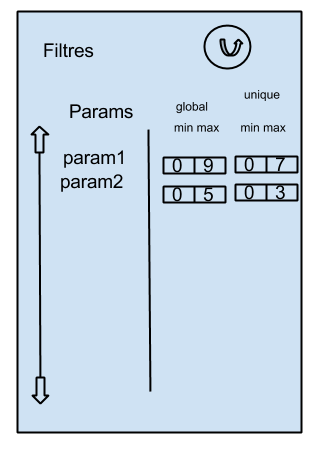
\includegraphics[width=0.25\textwidth]{figure/filtre.png}
			\end{center}
			\caption{Filtre}
			\label{fig:filtre}
		\end{figure}

		A l'heure actuelle, l'analyse d'arbre de grandes tailles à l'aide d'ADTool est difficile. En effet, ADTool a été pensé prioritairement pour la modélisation des systèmes sous forme d'ADTrees, et moins pour leurs analyses. ADTool met à disposition de l'expert, comme cela a été précisé précédemment, un certain nombre d'outils pour l'assister dans la modélisation de son système, parmi lesquels se trouve la valuation des noeuds de l'arbre. Une limite que présente ADTool est que, une fois le système à protéger complétement représenté sous la forme d'un ADTree, l'arbre peut être trop grand pour que l'expert puisse en retirer une information pertinante car le temps de parcours est trop long. 

		Le premier besoin qu'aura l'expert lors de l'analyse sera de rendre son arbre plus lisible, donc de le réduire. L'une des 

		En conséquence, l'analyse d'arbres à l'aide d'ADTool se fait principalement à la main, et devient donc impossible lorsque les arbres augmentent de tailles, faute à un support logiciel dédié.

		

		%\begin{itemize}
		  %\item bouton pour ajouter nouveau paramètre sur le filtre (par default : pas de filtre => pas de paramètres) 
			 % \begin{itemize}
			  	% \item ajouter ouvre selection de paramétres : menu déroulant précisant les paramètres disponibles.
			  %\end{itemize}
		  %\item tous les paramètres ont à coté d’eux deux sections : une de filtre global et une de filtre unitaire. Dans le filtre global sont présentes deux %cases, une nommée “min” et une nommée “max”. De même dans le filtre unitaire.
		 % \item par défaut, les min sont moins l'infini et les max sont l’infini (pas de filtre)
		  %\item il est possible d’inscrire des valeurs dans les cases “min” et “max” afin de réduire l’intervalle de sélection des branches de l'arbre.
		  %\begin{itemize}
			  	 %\item la section globale permet de conserver les branches de l’arbre dont la valeur totale du paramètre se trouve dans l’intervalle. (ex %: entre 500 et 1000 euros au total)
			  	% \item la section unitaire permet de conserver les branches de l’arbre dont chacune des valeurs de chacune des feuilles se trouve dans %l’intervalle. (ex : pas de dépenses de moins de 10 euros et pas de plus de 100 euros)
		 % \end{itemize}
		  %\item il est ainsi possible de combiner les critères de sélection (ex : entre 500 et 1000 euros au total et pas de dépenses de moins de 10 euros %et pas de plus de 100 euros ; et le temps entre X et Y et ….)
		 % \item barre de défilement pour les cas de surcharge de paramètres
		  %\item possibilité d'activer ou désactiver les paramètres ( bouton a cocher)
		  %\item bouton ``générer'' permet de créer un nouvelle arbre filtré en fonction des paramètres définie. Il est ouvert dans un nouvelle onglet de la %section ADTool de l'interface. 
		 % \item chaque arbre posséde son propre outil filtre. Lors de la génération, le nouvelle arbre posséde un outil filtre vide. 
		  %\item le nouvel arbre posséde un commentaire : filtre depuis l'arbre X avec paramétre Y, heure, version. \ldots
		  %\end{itemize}


	\subsection{Fonction de synthèse}
Il existe actuellement 6 valuations de synthèse dans ADTool, présentes dans le tableau ci-dessous.
		\begin{figure}
			\begin{center}
				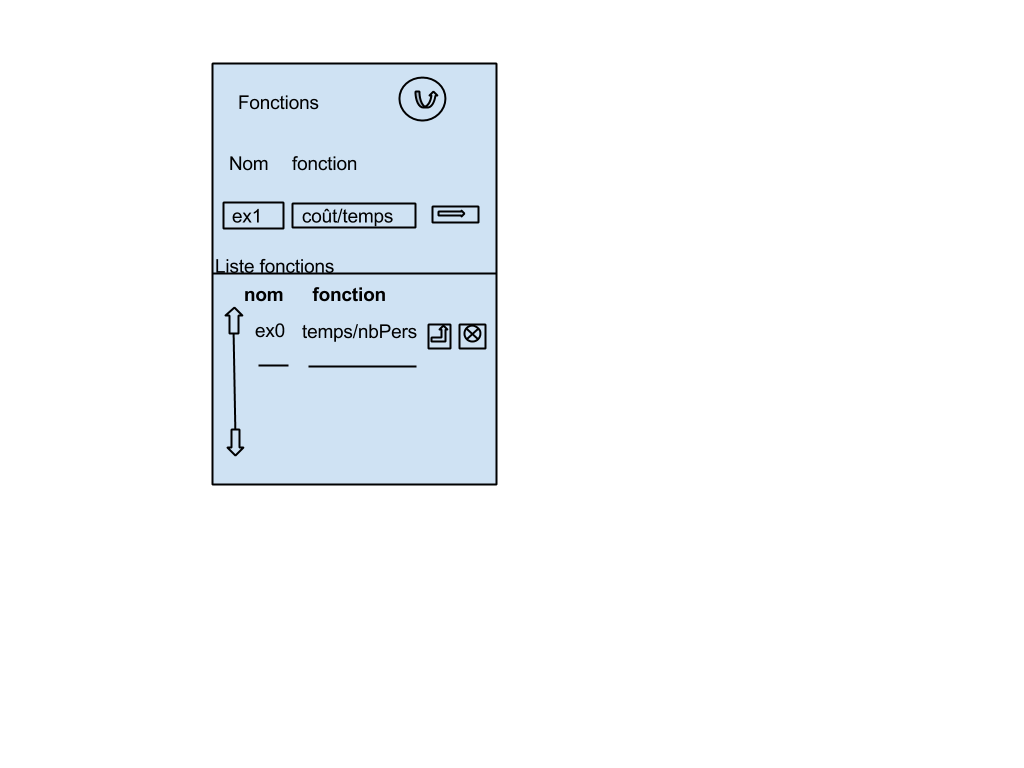
\includegraphics[width=0.25\textwidth]{figure/fonction.png}
			\end{center}
			\caption{Fonction}
			\label{fig:fonction}
		\end{figure}

L'utilisateur est 
		\begin{itemize}
			\item (présence préalable de 6 valuations de synthèse définies dans ADTool, et non instanciées par défaut. )
			\item décomposition en deux zones : une pour l'édition du nouveau paramètre et de sa fonction, et une pour le rappel des fonctions déjà existantes.
			\item Zone 1 : Présence d’un menu déroulant pour choisir laquelle des 6 valuation de synthèse est à instancier, et d'une zone textuelle pour écrire la fonction qu'on lui associe. La fonction est une fonction linéaire ou non, et qui prend en paramètres des valuations de l'arbre déjà définies (dans ADTool ou d'autres fonctions de synthèse). Bouton à coté pour valider la création. Si echec de la création (fonction non valable, etc.), message d'erreur donné par le guide (avec conseils éventuels).
			\item zone 2 : présence en dessous de la zone 1 d’une zone de rappel des fonctions de synthèse déjà instanciées. A coté de chacune d’entre elles il y a deux boutons : un pour modifier une fonction déjà créée, et un autre pour la supprimer.
			\item bouton “actualiser” en haut pour mettre à jour la liste des fonctions. \ldots
		\end{itemize}
		
		
		

